

本章中构建的软件并不复杂——我们将创建一个简单的计算器,将两个数字相加(图12.1)。作为一个控制台应用程序发布,带有文本用户界面和一个用于执行数学运算的库,这可能用于其他项目。虽然在现实中没有太多用处,但它将用于探索本书中讨论的所有技术,以及如何在实践中进行协同工作:

\begin{center}
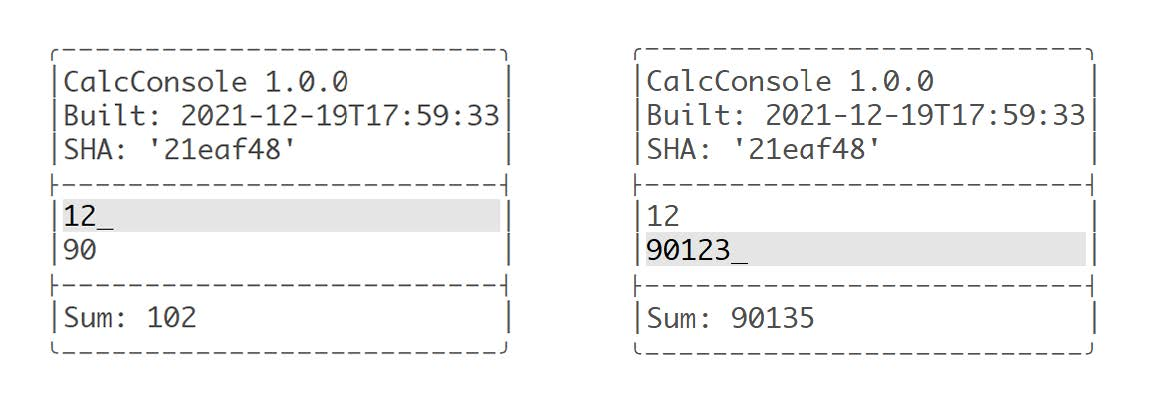
\includegraphics[width=0.8\textwidth]{content/3/chapter12/images/1.jpg}\\
图12.1 控制台计算器用户界面的两种状态
\end{center}

通常,项目要么生成面向用户的可执行文件,要么为开发人员生成库。同时具备这两种功能的项目很少见——一些应用程序提供独立的SDK或库来支持插件,另一种情况是提供其用法示例的库。我们在本章中构建的项目在某种程度上属于最后一类。

这里先回顾一下之前章节的内容,并选择相应的技术和工具来构建应用:

\textbf{第1章:}

提供关于CMake的基本信息——如何安装它,并使用命令行来构建项目。这里提供的有关项目文件的信息是关键:不同文件的职责、常规使用的名称,以及一些奇淫技巧。本章中,还讨论了生成器的预设文件,但在本项目中先跳过这些文件。

\textbf{第2章:}

介绍了编写正确的列表文件和脚本所需的工具,分享了关于代码的基本信息:注释、命令调用和参数。我们还详细解释了变量、列表和控制结构,并给出了一些非常有用的命令。这些知识将应用于整个项目。

\textbf{第3章:}

这里的内容将对项目产生关键性影响:

\begin{itemize}
\item 
指定最低的CMake版本将决定应用哪些CMake策略,命名、版本控制和配置项目语言会影响构建的基本行为。

\item 
了解形成目录和文件布局的项目分区和结构。

\item 
系统可以帮助我们处理不同的环境,特别是对于这个项目——例如,是否需要运行ldconfig?

\item 
工具链配置允许C++和编译器支持特定的标准需求。
\end{itemize}

本章还说明了禁用源内构建的原因。

\textbf{第4章:}

这里,强调了每个现代CMake项目如何使用目标,原因如下:

\begin{itemize}
\item 
定义一些库和可执行程序(用于测试和生产)将使项目保持有组织和DRY。

\item 
目标属性和传递性使用需求(传播属性)保持配置接近目标定义。

\item 
生成器表达式将在整个解决方案中出现,使它们尽可能简单。
\end{itemize}

这个项目中,将使用自定义命令为Valgrind和覆盖率报告生成文件,并且使用目标钩子(PRE\_BUILD),来清理覆盖率工具生成的.gcda文件。

\textbf{第5章:}

没有编译就没有C++项目,CMake可以以多种方式调整这个过程:扩展目标的源、配置优化器和提供调试信息。对于这个项目,默认的编译标志就可以了,但我们将继续使用预处理器:

\begin{itemize}
\item 
在编译后的可执行文件中存储构建元数据(项目版本、构建时间和Git提交SHA),并将其显示给用户。
	
\item 
将启用头文件的预编译。在如此小的项目中,这并不是必须的,但会帮助我们实践这个知识点。
\end{itemize}

统一构建不是必要的——这个项目不够大,但也可以添加。

\textbf{第6章:}

提供了关于链接的信息(在任何项目中都很有用),其中大部分在默认情况下很有用。但是由于这个项目也提供了一个库,将显式地引用以下的一些构建说明:

\begin{itemize}
\item 
用于测试和开发的静态库

\item 
要发布的动态库
\end{itemize}

本章概述了如何分离main()进行测试,我们的项目中也有测试。

\textbf{第7章:}

为了使项目更有趣,将引入一个外部依赖项:文本UI库。本章中描述了一些依赖管理方法。选择正确的一个并不太难:FetchContent实用程序模块通常是推荐的,也是最方便的(除非解决本章中描述的特定情况)。

\textbf{第8章:}

必须有适当的自动化测试,以确保解决方案的质量不会随着时间而下降。我们将添加对CTest的支持,并为测试正确地构造项目(将应用前面提到的main()分离)。

此外,还讨论了两个测试框架:Catch2和GTest;对于这个项目,我们将使用后者。为了获得关于覆盖率的明确信息,将生成带有LCOV的HTML报告。

\textbf{第9章:}

要执行静态分析,可以从各种各样的工具中进行选择:Clang-Tidy、Cpplint、Cppcheck、include-what-you-use和连接其他工具。本例中,将使用Cppcheck,因为Clang-Tidy不能很好地处理用GCC编译的预编译头文件。动态分析将使用Valgrind的Memcheck工具完成,将使用Memcheck封面包装器生成HTML报告,源代码也将在编译过程中使用ClangFormat自动格式化。

\textbf{第10章:}

因为提供一个库作为这个项目的一部分,所以要提供一些与之配套的文档。CMake可以用Doxygen自动生成,所以可以通过添加doxygenawesome-css来进行更新文档外观。

\textbf{第11章:}

最后,配置解决方案的安装和打包,将按照描述准备文件以形成包,以及目标定义。我们将通过包含GNUInstallDirs模块,将其和构件从构建目标安装到适当的目录中。我们将另外配置一些组件模块化,并与CPack一起使用。

专业项目还附带一些文本文件:README、LICENSE、INSTALL等。我们会在最后简要地讨论这个问题。

\begin{tcolorbox}[colback=blue!5!white,colframe=blue!75!black,title=Note]
为了使事情更简单,不会实现检查所有必需的实用程序和依赖项是否可用的逻辑。我们将在这里依赖CMake来显示诊断,并告诉用户缺少什么。若在阅读本书后发布的项目获得了其他人的关注,可能就需要考虑添加这些机制来改善用户体验了。
\end{tcolorbox}

形成了一个清晰的计划之后,再从逻辑目标和目录结构两方面讨论实际的构建项目。
















